\documentclass{beamer}
\usepackage[utf8]{inputenc}

\usepackage{amsmath,amsfonts,amssymb,amsthm,
mathtools,mathrsfs}
\usepackage{physics}
\usepackage{xcolor}
\usepackage{listings}
\usepackage{caption, subcaption}
\usepackage{pgf-pie}
\usepackage{hyperref}

\usetheme{Madrid}
\usecolortheme{default}
\useoutertheme[subsection=false]{miniframes}

\addtobeamertemplate{block example begin}{%
    \setlength{\textwidth}{0.8\textwidth}
}{}

\usepackage[style=apa, backend=biber, natbib]{biblatex}
\addbibresource{references.bib}


\title[LSD Analysis]{Liquidity Unleashed: A Research-driven Analysis of Post-Shanghai LSDs}
\subtitle{ETHChicago 2023}
\author[Mingxuan He]{
    Mingxuan He\\ 
    mingxuanh.eth
    }


\institute[]{
Phoenix graduate scholar (computational economics), University of Chicago\\
Research fellow, Nethermind
}


\date{\today}


% table of contents page before each section (optional)
% \AtBeginSection[]
% {
%   \begin{frame}
%     \frametitle{Table of Contents}
%     \tableofcontents[currentsection]
%   \end{frame}
% }


\begin{document}

% title page
\begin{frame}
\titlepage  
\end{frame}

% table of contents
\begin{frame}
\frametitle{Table of Contents}
\tableofcontents
\end{frame}


%----------------
\section[Introduction]{Introduction to Ethereum Staking \& LSDs}
\begin{frame}{History of Ethereum Staking}

    \begin{itemize}
        \item The Merge (Sep 2022): Ethereum migrated from PoW to PoS\\
        $\Rightarrow$ Now anyone can stake $32\Xi$ on mainnet and accrue rewards as a validator
        \bigskip
        \item The Shapella/Shanghai Upgrade (Apr 2023) \\
        $\Rightarrow$ Introduced option to withdraw staked ETH (unstake)
    \end{itemize}

    
\end{frame}

\begin{frame}{Breakdown of Ethereum Staking Rewards}
\begin{itemize}
    \item Consensus layer rewards: Attestation, block proposal, sync committee
    \item Execution layer rewards: Txn fee (EIP-1559), MEV
\end{itemize}
\begin{figure}
    \centering
    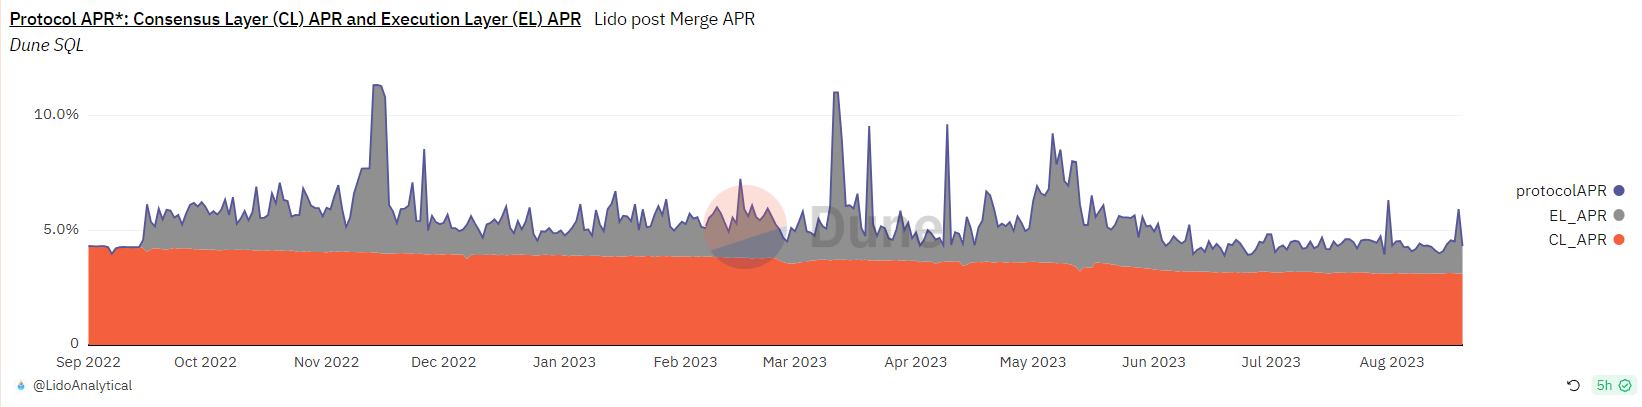
\includegraphics[width=\textwidth]{figures/lido_apr.png}
\end{figure}
\tiny{source: \href{https://dune.com/LidoAnalytical/lido-execution-layer-rewards}{@LidoAnalytical on Dune}}

\end{frame}



\begin{frame}{ETH Staking Landscape}
    \begin{figure}
        \centering
        \begin{subfigure}[b]{0.45\textwidth}
            \centering
            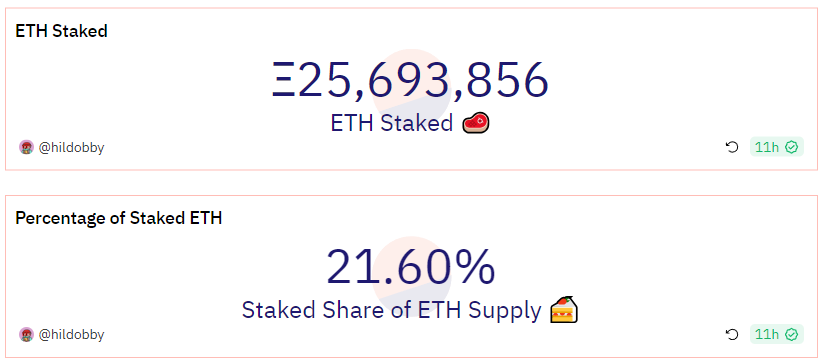
\includegraphics[width=\textwidth]{figures/eth_stake_stats.png}
        \end{subfigure}
        \begin{subfigure}[b]{0.45\textwidth}
            \centering
            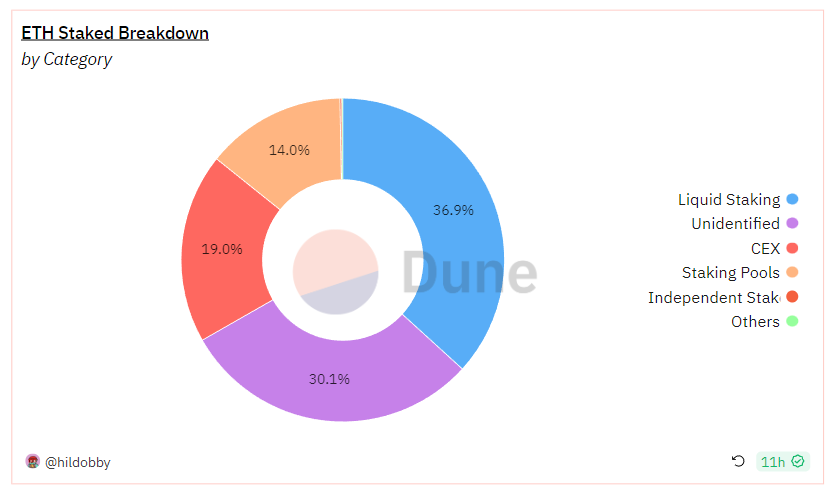
\includegraphics[width=\textwidth]{figures/eth_stake_breakdown.png}
        \end{subfigure}
    \end{figure}
    \tiny{source: \href{https://dune.com/hildobby/eth2-staking}{@hildobby on Dune}}

\end{frame}

\begin{frame}{Liquid Staking Derivatives (LSDs)}
    Actors: stakers, staking pools, node operators
    \begin{enumerate}
        \item Stakers deposit ETH into staking pools in exchange for LSDs
        \item Staking pools delegate batches of $32\Xi$ to NOs to run Ethereum validators and earn staking rewards
        \item LSDs can be traded on AMMs, used as DeFi collateral, etc.
        \item LSDs are redeemable for ETH at any time
    \end{enumerate}
    \bigskip
    Most LSDs accrue rewards automatically i.e. \textbf{holding LSDs is equivalent to staking ETH in the pool}
\end{frame}

\begin{frame}{LSDs saw huge growth after Shapella}
    \begin{figure}
        \centering
        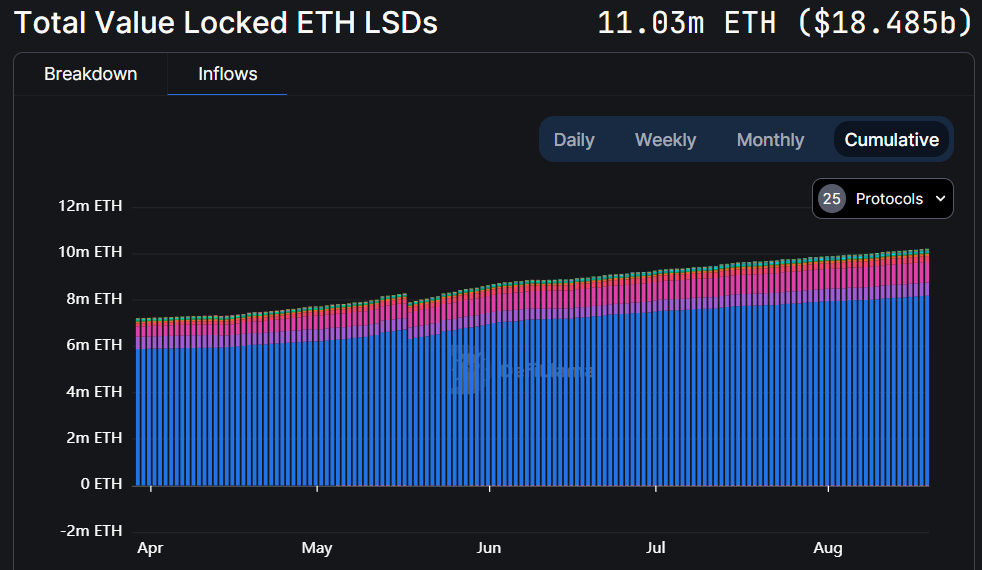
\includegraphics[width=0.8\textwidth]{figures/lsd_2023.png}
    \end{figure}
    \tiny{source: \href{https://defillama.com/lsd}{DeFi Llama}}
    
\end{frame}

%----------------
\section{Economic Analysis}
\begin{frame}{Liquid Staking Pools as Banks}

    \footnotemark Banks are financial intermediaries which creates liquidity by:

    \begin{itemize}
        \item Holding liquid funds (e.g. customer deposits) as liabilities
        \item Investing in illiquid investment projects (e.g. loans, bonds) as assets
    \end{itemize}

    % use columns
    \begin{tabular}{|c|c|c|}
        \hline
         & Banks & Liquid Staking Pools \\
        \hline
        Invests in & Loans & ETH validators \\
        \hline
        Deposits & Checking accounts & ETH deposits \\
        \hline
    \end{tabular}

\footnotetext{Diamond and Dybvig (1983) Theory of Banking}
\end{frame}

\begin{frame}{Supply and Demand Analysis}
    
\end{frame}

\begin{frame}{How Liquid are LSDs, Really?}
    Introducing quantitative measures of liquidity\\
    queues
\end{frame}


\begin{frame}{Risks}
    \begin{itemize}
        \item Liquidity risk: e.g. CRV exploit July 2023
        \item Price risk: e.g. ETH price drop
        \item Bank runs
    \end{itemize}
\end{frame}


\begin{frame}{More Risks}
    \begin{itemize}
        \item APR drop
        \item Inflationary ETH
    \end{itemize}
\end{frame}

%----------------
\section{Research Insights}

\begin{frame}{LSD Risk Simulations}
    
\end{frame}

\section*{}

\begin{frame}[allowframebreaks]{References}
    \nocite{*}
    \printbibliography
\end{frame}


\end{document}
